The measurements of $R_K$ and $R_K^*$ in the low $q^2$ 
and central $q^2$ regions currently represent the most 
precise tests of Lepton Flavour Universality (LFU). 
Contrary to previous measurements, this analysis aligns 
with the Standard Model predictions, with an agreement of 
$\num{0.2}\sigma$, as shwon in figure \ref{fig:results}. 
This study underscores the importance of understanding 
electron misidentification and also demonstrates the 
benefits of a double-ratio approach in minimizing 
systematic uncertainties. The statistical uncertainties 
significantly outweigh the systematic ones in this 
analysis, suggesting that a larger dataset is required 
to improve the precision of the measurement.

\begin{figure}
    \centering
    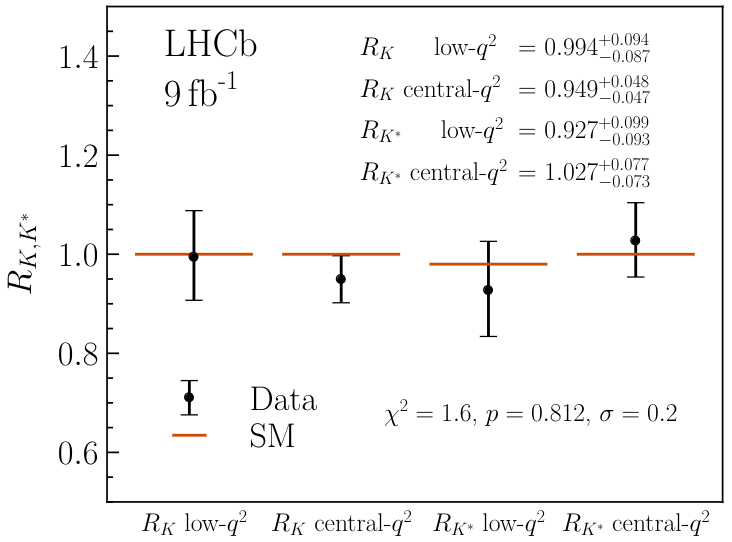
\includegraphics[width=\linewidth]{figures/results.png}
    \caption{Graphical comparison of the measured results of $R_K$ and $R_{K^*}$ in the low and central $q^2$ range with the standard model \cite{lhcbcollaboration2022measurement}.}
    \label{fig:results}
\end{figure}

While the LFU tensions with respect to the Standard Model 
appear to be of systematic origin, the tensions related to 
the branching fractions $\mathcal{B}(B^{(0,+)}\to K^{(+,*0)}l^+l^-)$ 
 \cite{Branchingfraction}.

The upcoming LHCb Run 3, with its increased statistics and 
new detector enhancements, including the trigger system, is 
expected to further refine the precision of LFU tests.